\chapter*{Úvod}
\addcontentsline{toc}{chapter}{Úvod}

Na internetu je dnes možné najít téměř cokoli, kupříkladu stav počasí, encyklopedické informace, odborné publikace, jízdní řády a podobně. Tyto informace jsou uloženy jako webové stránky systému WWW (World Wide Web) a kterýkoli uživatel internetu má k nim přístup a může z nich čerpat.

Pro lidi je systém WWW vyhovující zdroj informací, nicméně narazíme na problém, pokud chceme tyto informace číst strojově. WWW totiž nepopisuje, jak by měly být informace na internetu prezentovány. Každý publikovatel si může data zveřejnit jinak, například tabulkou, odrážkovým seznamem, nebo ve větách. Tyto informace jsou stále snadno čitelné pro člověka, ale obtížně čitelné pro stroj.

Možností řešení tohoto problému je zveřejňovat data i ve strojové podobně. Nabízí se například tabulky ve formátu CSV, nebo komplikovanější data ve formátu JSON a XML. Zde je již snadné číst data a dál je zpracovávat, ale programátor je stále nucen pochopit a přizpůsobit program na rozhraní těchto dat.

Konečným řešením se nabízí popsat data pomocí RDF frameworku, jež je popsán důkladněji v následující kapitole.

\bigskip

Tato práce se zabývá reprezentací dat popsancýh právě pomocí RDF. RDF reprezentuje entity z reálného světa jako vrcholy grafu a jejich vlastnosti pomocí hran propojující tyto entiy. Data uložená v grafových databázích jsou snadno čitelná počítačovými programy a je jednoduché propojovat různé datové zdroje do větších a provádět nad nimi dotazy.

Jako veškerá strojová data je potřeba i tyto grafová data vizualizovat. Příkladem může být datový analytik, který se chce přesvědčit, že jsou data uložena tak, jak bylo zamýšleno.

Jako modelový příklad vizualizace uveďme entitu Karla Čapka a některá jeho data, jež má o něm uložená Wikipedie.

\begin{figure}[h]
    \centering
    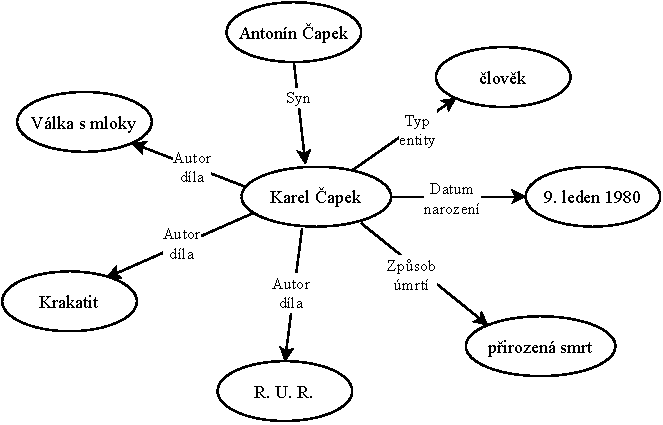
\includegraphics{media/capek-full.pdf}
    \caption{Ukázka části grafu jež může reprezentovat Karla Čapka.}
    \label{fig:capek-full}
\end{figure}

Jak vidíme z obrázku \ref{fig:capek-full}, zobrazit všechna data k uzlu může být velmi nepřehledné a takovýchto dat může být stovky. Pokud nás například zajímají pouze díla Karla Čapka, určitě v grafu nebudeme chtít mít informaci, že Karel Čapek je člověk. Možností řešení tohoto problému je dívat se na entity pouze určitým pohledem a tedy zobrazit pouze ty vztahy k vrcholu, jež odpovídají pohledu.

Kupříkladu pokud bychom chtěli procházet rodokmenem, je vhodné se na Karla Čapka dívat jako na osobu, jež má rodiče a sama může být rodičem ostatních osob. V tuto chvíli nás nezajímají ostatní vlastnosti jako knihy, které napsal, nebo ocenění, která získal. Na Karla Čapka se ale můžeme dívat i jako na spisovatele, kde nás pak zajímají pouze jeho díla a rodinné vztahy můžeme skrýt. Příklad tekovýchto pohledů je na obrázku \ref{fig:capek-part}.

\begin{figure}[h]
    \centering
    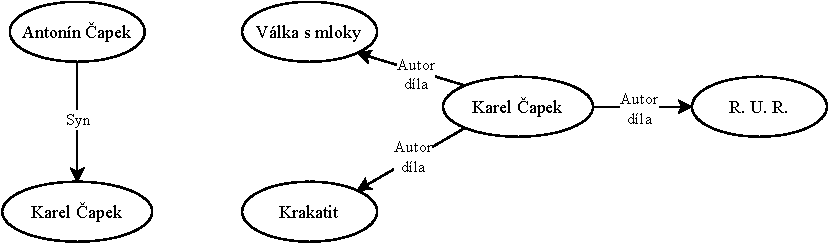
\includegraphics{media/capek-part.pdf}
    \caption{Pohled na Karla Čapka jako na osobu mající rodinu (vlevo) a na spisovatele jež je autorem literárních děl (vpravo)}
    \label{fig:capek-part}
\end{figure}

Tento způsob procházení grafových dat sice vyžaduje předem nadefinovat pohledy, ale procházení dat je pak jednoduché a velmi přehledné.

\section{Cíl práce}

Cílem této práce bylo vyrobit webovou aplikaci, jež by na základě předem definovaných pohledů vizualizovala grafová data a umožňovala uživateli procházet tento graf a objevovat nové vrcholy. Protože je žádoucí mít více pohledů na konkrétní typ vrcholu, pohledy jsou seskupeny do takzvaných konfigurací. Konfigurace pak popisuje nejen pohledy na různé typy vrcholů, ale i jaké vrcholy lze takto vizualizovat a z jakých zdrojů čerpat.

Konfigurace, jež jsou použité v aplikaci jsou například:
\begin{itemize}
    \item \textbf{Procházení živočichů na Wikidatech} - Uživatel může vizualizovat jednotlivé rostlinné a živočičné druhy a procházet je podle rozdělení do taxonů.
    \item \textbf{Procházení slavných osobností z Wikidat} - Uživatel může procházet slavné osobnosti a nechat si načíst jejich filmová a literární díla a rodinné vztahy.
\end{itemize}

Kromě procházení si bude uživatel moci zobrazit detailní informace ke konkrétnímu vrcholu v závislosti na pohledu.
